
\documentclass{article}
\usepackage{graphicx}  % For including images
\usepackage{geometry}  % For adjusting margins and spacings
\usepackage{enumitem}
\usepackage{float}
\usepackage{tabularx} % for flexible column width
\usepackage{array} % for centering content in cells


\usepackage{fancyhdr}
\pagestyle{fancy}
\fancyhf{} % Clear all headers and footers
\renewcommand{\headrulewidth}{0.4pt} % Add a rule below the header


\lhead{Name: Christopher Nowacki}
\chead{Class: CIS 280}
\rhead{Assignment: Module 6}
% Adjust page margins
\geometry{top=2.5cm, bottom=2cm, left=2cm, right=2cm, headheight=15pt}

\begin{document}
\thispagestyle{fancy}
\section{Part I}
\begin{enumerate}
    % Question 1
    \item \textbf{What is O-O analysis?}
    
    Objected Oriented Analysis describes an information system via object identification. This gives you an overview of what entities, functions, messages, and transactions, and data will be required to create the information system. 

    % Question 2
    \item \textbf{Define an object in an information system and provide three examples.}
    
    An object represents a person, place, item, event, or transaction. It contains attributes and/or methods.
    \begin{enumerate}[leftmargin=2cm]
      \item Object: Librarian
      \item Object: Library
      \item Object: Book Reading
    \end{enumerate}

    % Question 3
    \item \textbf{Define an attribute and provide three examples.}

    An \textbf{attribute} is a characteristic that describes an object.
    \begin{enumerate}[leftmargin=2cm]
      \item Object: Librarian \\ 
            Attributes: \textit{Name, Employee\_ID}
      \item Object: Library \\
            Attributes: \textit{Name, Location, Location\_ID, Open?}
      \item Object: Book Reading \\
            Attributes: \textit{Reader, Date, Time}
    \end{enumerate}

    % Question 4
  \item \textbf{Define a \textit{method} and provide three examples}

  \textbf{Methods} are functions that the object performs when it receives a message.
    \begin{enumerate}[leftmargin=2cm]
      \item Object: Librarian \\
            Methods: \textit{Update Book Status, Issue Library Card}
      \item Object: Library \\
            Methods: \textit{Schedule Event, List Events, Change Hours}
      \item Object: Book Reading \\
            Methods: \textit{Add Reading, Delete Reading, Update Reading}
    \end{enumerate}

    % Question 5
  \item \textbf{Define \textit{encapsulation} and explain how it is used in OO analysis.}

    With \textbf{encapsulation}, \textit{data and functions are self-contained} in an object class.
    IT is useful in the OOP concept as it allows objects to be used as modular components
    and prevents its internal code from being changed.

    % Question 6
  \item \textbf{Define a \textit{class, subclass, and superclass} and provide three examples of each.}

  A \textbf{class} is a blueprint for creating \textit{objects}. A \textbf{subclass} is a class that
    inherits the properties from another class, called a \textbf{superclass} or \textbf{parent class}.
    \\ \\
    \textit{class} \textbf{record} in \textit{superclass} \textbf{recorded media} \\
    \textit{class} \textbf{7"} in \textit{superclass} \textbf{record} \\
    \textit{class} \textbf{12"} in \textit{superclass} \textbf{record} \\ \\
    
    Superclass would be \textbf{recorded media}, it's \textit{child class} in this case would be
    \textbf{record, cassette, cd, etc}. \\

    \textbf{record} would be the \textit{parent class} for: \textbf{7", 10", 12", etc}, making the
    mentioned record sizes the \textbf{subclass}.

    % Question 7
  \item \textbf{Explain the concept of \textit{inheritance} in object relationships.}
    \textbf{Inheritance} enables an object to derive one or multiple attributes from its \textbf{parent class}.
    The class inheriting the attributes is the \textbf{child class}.

    For example, an \textbf{animal} class could have methods like eat\_food() and drink\_water(), and a 
    \textbf{tiger} subclass could inherit those methods.

    % Question 8
  \item \textbf{Draw an \textit{object relational diagram} for a typical library system.}
    \begin{figure}[H]
      \centering
      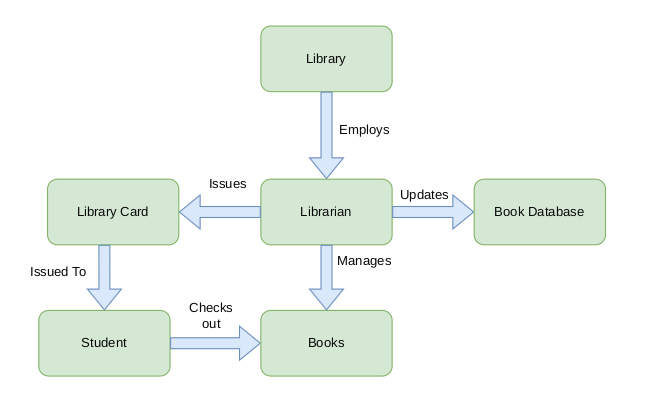
\includegraphics[width=0.8\linewidth]{../images/object_relational_diagram.png}
      \caption{Objected Relational Diagram}
    \end{figure}

    % Question 9
  \item \textbf{Define a \textit{use case} and a \textit{use case diagram} and prepare a sample of each.}
    
    A \textbf{use case} is a description of a way that a user can interact with a system or product. \\
    A \textbf{use case diagram} is a visual diagram that shows the process, entities, and "touch points",
    i.e. where an entity is involved in a process.

  \begin{table}[h]
    \centering
    \begin{tabularx}{\textwidth}{|l|X|}
        \hline
        \textbf{Use Case Name} & Checkout Book \\
        \hline
        \textbf{Actor} & \textbf{Librarian}, \textit{Student} \\
        \hline
        \textbf{Preconditions} & \textit{Student} has \textbf{library card} \\
        \hline
        \textbf{Postconditions} & \textbf{book} status is changed to \textit{checked out} \\
        \hline
        \textbf{Description} & A student wants to check out a book, and the Librarian helps check it out to them manually. \\
        \hline
        \textbf{Steps} & 
        \begin{tabular}{ll}
        1.1. & Student selects book for checkout. \\
        1.2. & Librarian confirms that the book is available for checkout. \\
        1.3. & Librarian confirms there are no holds on student's account. \\
        1.4. & Library updates book status to \textbf{CHECKED OUT}. \\
        1.5. & Student is issued a receipt with a \textbf{DUE BY} date.
        \end{tabular} \\
        \hline
        \textbf{Alternate Flow} & 
        1.3.1. If Student has holds on account, they must settle holds before more books can be checked out. \\
        \hline
    \end{tabularx}
    \caption{Use Case Definition for "Checkout Book"}
    \label{tab:use-case-checkout}
\end{table}
  \begin{figure}[H]
    \centering
    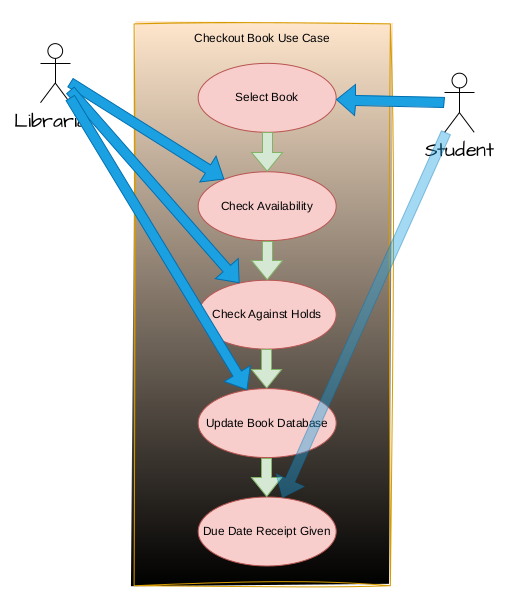
\includegraphics[width=0.8\linewidth]{../images/use_case_book_checkout.png}
    \caption{Book Checkout Use Case Diagram}
  \end{figure}

    % Question 10
  \item \textbf{Why is it important to use a modeling tool and not just a diagramming tool during O-O analysis?}

  Modeling tools provide a solutions to assist analysts in documenting system components. They also
  improve modularity. Once an object is described in one section, it can be reused with little extra 
  effort, where in a diagramming tool you would have to re-draw and create the link every time. A modeling
  tool will also adhere to UML guidelines so it will be harder to "break the rules".
    % insert img
  % \begin{figure}[H]
  %  \centering
  %  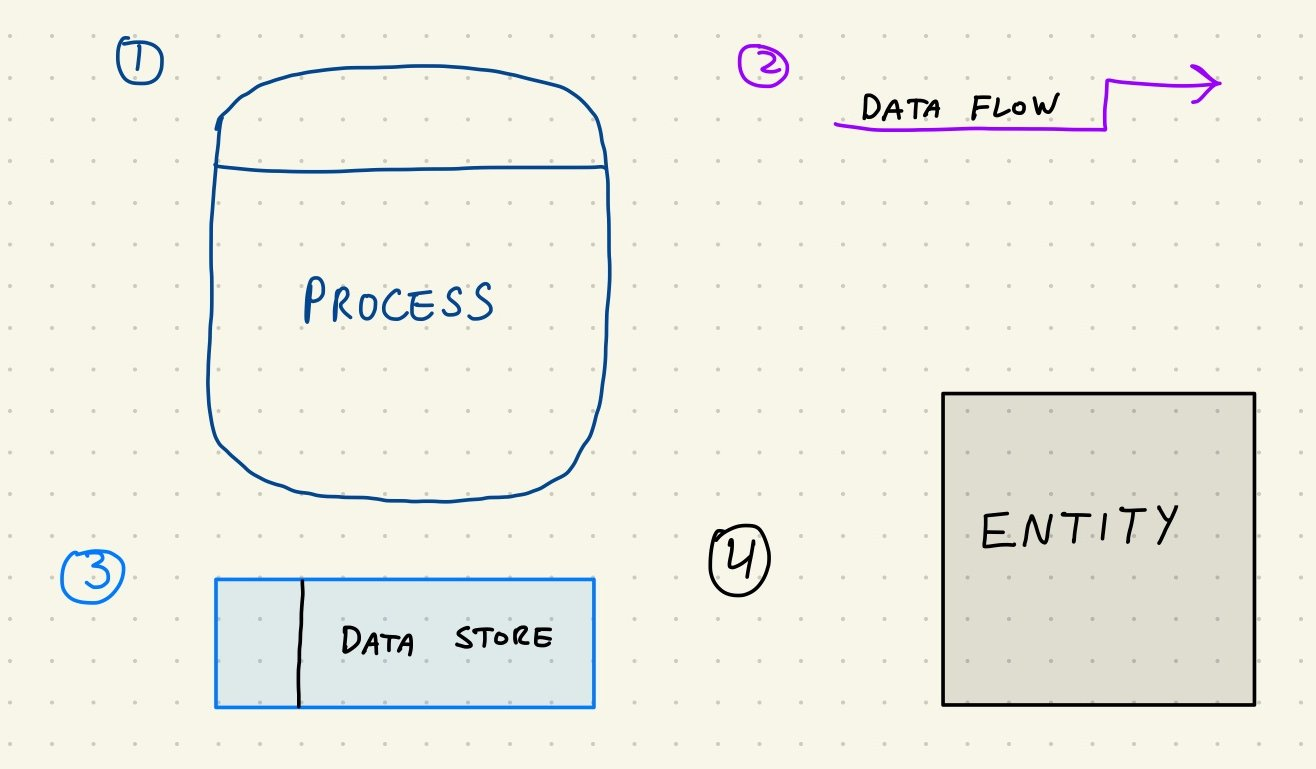
\includegraphics[width=0.8\linewidth]{dfd_symbols.jpg}
  %  \caption{DFD symbols}
  %\end{figure}


\newpage

\section{Part II}

\subsection{Use Cases/Use Case Diagram}

% Schedule an Appointment Use Case
\begin{table}[h]
    \centering
    \begin{tabularx}{\textwidth}{|l|X|}
        \hline
        \textbf{Use Case Name} & Schedule an Appointment \\
        \hline
        \textbf{Actor} & \textbf{Patient}, \textit{Admin} \\
        \hline
        \textbf{Preconditions} & 
        \begin{itemize}
            \item The doctor's schedule is open.
            \item Patient's records are accessible to the admin.
        \end{itemize} \\
        \hline
        \textbf{Postconditions} & Appointment is scheduled and both the patient and doctor have details of appt. \\
        \hline
        \textbf{Description} & A patient wishes to schedule an appointment with a doctor. The patient can either call the office and the admin will schedule it, or the patient can use the online portal to book it. \\
        \hline
        \textbf{Steps} & 
        \begin{tabular}{ll}
            1.1 & Patient contacts the office or accesses the online portal. \\
            1.2 & Patient provides desired date and time or selects from available slots. \\
            1.3 & Administration checks doctor's availability. \\
            1.4 & Appointment is scheduled. \\
            1.5 & Patient received a confirmation.
        \end{tabular} \\
        \hline
        \textbf{Alternate Flow} & 
        \begin{tabular}{ll}
            1.3.1 & During step 1.3., admin finds doctor has no open appointments available. \\
            1.3.2 & Admin offers alternate provider. \\
            1.3.3 & Patient selects a new slot or does not move forward with booking. \\
            1.3.4 & If new slot is selected, proceed to step 1.4 of the basic flow.
        \end{tabular} \\
        \hline
        \textbf{Exceptions} & 
        \begin{itemize}
            \item If the system or online portal malfunctions, patient will be advised to contact later or use another method of booking.
            \item If the doctor is on an extended leave, admin might suggest scheduling with an alternate physician.
        \end{itemize} \\
        \hline
    \end{tabularx}
    \caption{Use Case Definition for "Schedule an Appointment"}
    \label{tab:use-case-appointment}
\end{table}

% Update Medical Information Use Case
\begin{table}[H]
    \centering
    \begin{tabularx}{\textwidth}{|l|X|}
        \hline
        \textbf{Use Case Name} & Update Medical Information \\
        \hline
        \textbf{Actor} & \textbf{Patient}, \textit{Admin} \\
        \hline
        \textbf{Preconditions} & 
        \begin{itemize}
            \item Patient has an account within the system. 
        \end{itemize} \\
        \hline
        \textbf{Postconditions} & Medical information is up-to-date. \\
        \hline
        \textbf{Description} & Patient's medical profile is out-of-date, and needs to be updated. Patient can log-in and update through a portal, or could fill out updated information at their next in office visit via pen and paper, which will be manually updated by admin. \\
        \hline
        \textbf{Steps} & 
        \begin{tabular}{ll}
            1.1 & Patient comes into the office for a visit or logs into the portal. \\
            1.2 & Patient updates and saves medical history and billing details. \\
            1.3 & Notification of update is sent to administration. \\
            1.4 & Administration reviews the changes and confirms updated details in the system.
        \end{tabular} \\
        \hline
        \textbf{Exceptions} & 
        \begin{itemize}
            \item If the online system malfunctions, admin will encourage patient to update the information at their next visit or try again later.
        \end{itemize} \\
        \hline
    \end{tabularx}
    \caption{Use Case Definition for "Update Medical Information"}
    \label{tab:use-case-update}
\end{table}

\newpage
Use Case Diagram for \textit{X-Ray Procedure}

\begin{figure}[H]
  \centering
  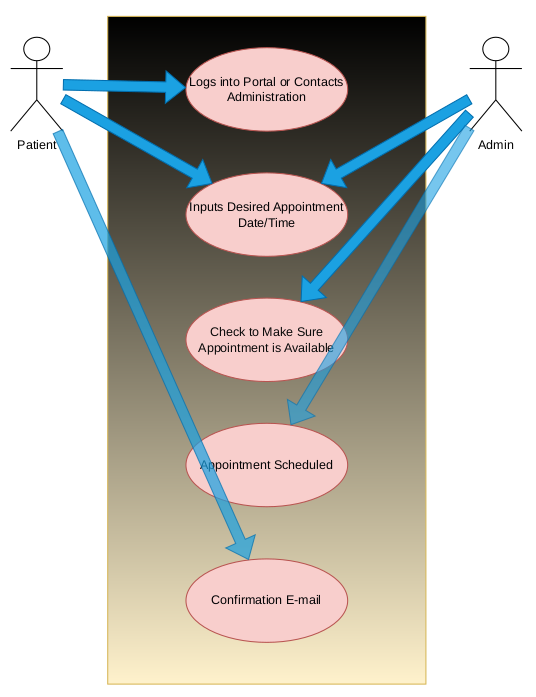
\includegraphics[width=0.8\linewidth]{../images/use_case_diagram_pcp.png}
  \caption{Use Case Diagram}
\end{figure}
\newpage
\subsection{Domain Class Diagram}

Domain Class Diagram for \textit{Appointment Booking}.

\begin{figure}[H]
  \centering
  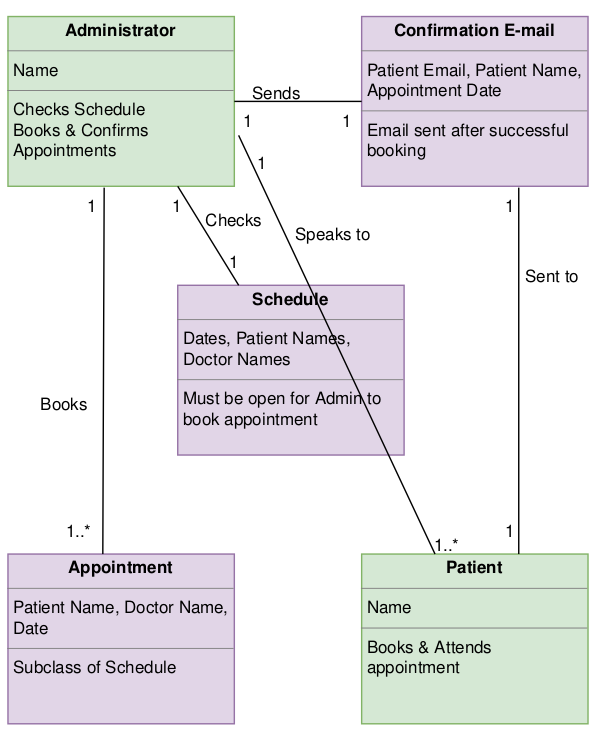
\includegraphics[width=0.8\linewidth]{../images/domain_class_diagram.png}
  \caption{Domain Class Diagram}
\end{figure}

\newpage
\subsection{Sequence Diagram}

Sequence Diagram for \textbf{Appointment Booking}

\begin{figure}[H]
  \centering
  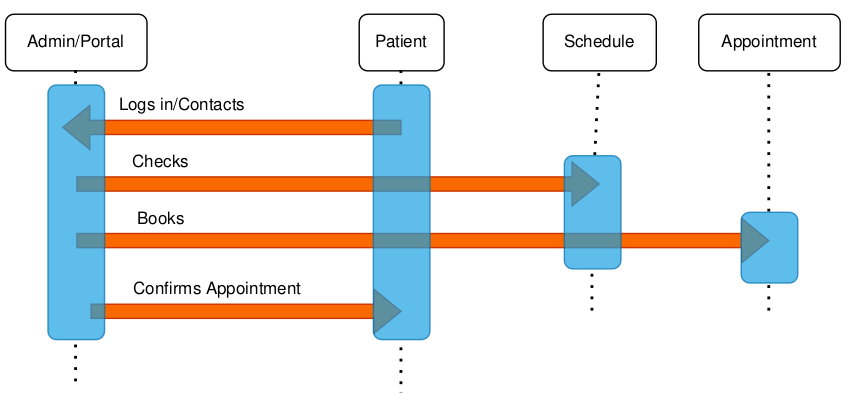
\includegraphics[width=0.8\linewidth]{../images/sequence_diagram.png}
  \caption{Sequence Diagram}
\end{figure}

\subsection{State Transition Diagram}

State Transition Diagram for Appointment Booking

\begin{figure}[H]
  \centering
  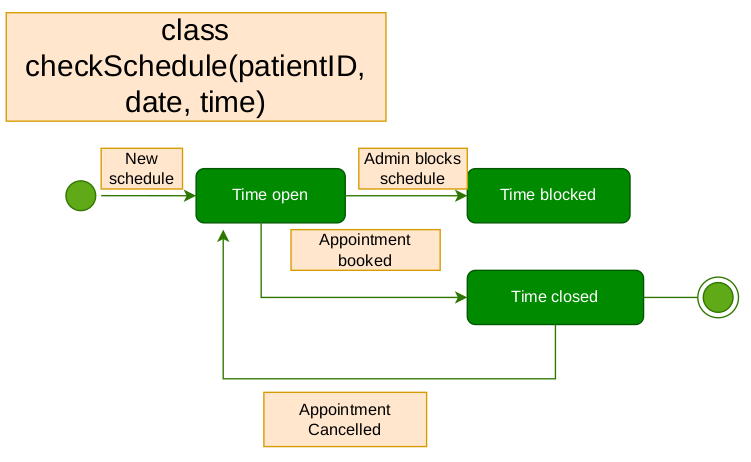
\includegraphics[width=0.8\linewidth]{../images/state_transition_diagram.png}
  \caption{State Transition Diagram}
\end{figure}

\newpage
\subsection{Activity Diagram}

Activity Diagram for Appointment Booking

\begin{figure}[H]
  \centering
  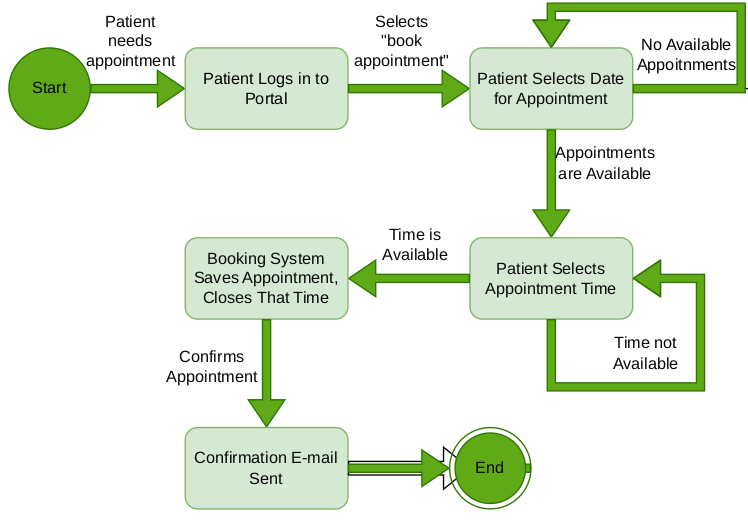
\includegraphics[width=0.8\linewidth]{../images/activity_diagram.png}
  \caption{Activity Diagram}
\end{figure}


% Repeat the above pattern for DFD 2, DFD 3, and DFD 4
\end{enumerate}
\end{document}

